\chapter{Modeling and simulation with \adevs}
\label{chapter:intro}
\adevs\ is a simulator for models described in terms of the Discrete Event System Specification (DEVS)\footnote{A comprehensive introduction to the Discrete Event System Specification can be found in ``Theory of Modeling and Simulation, 2nd Edition" by Bernard Zeigler \textit{et. al.}, published by Academic Press in 2000.} The key feature of models described in DEVS (and implemented with \adevs) is that their dynamic behavior is defined by events. An event is any change that is significant within the context of the model being developed.

The modeling of discrete event systems is most easily introduced with an example. Suppose we want to model the checkout line at a convenience store. There is a single clerk who serves customers in a first come-first served fashion. The time required for the clerk to ring up each customer's bill depends on the number of items purchased. We are interested in determining the average and maximum amount of time that customers spend waiting in line at the clerk's counter.
\begin{figure}[ht]
\centering
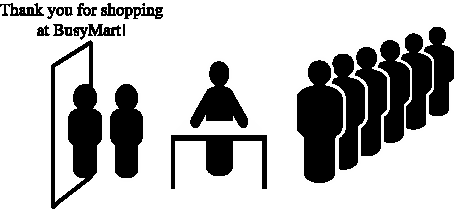
\includegraphics{intro_figs/busy_mart.pdf}
\caption{Customers waiting in line at BusyMart.}
\label{fig:busy_mart}
\end{figure}

To simulate this system, we need an object to represent each customer in the line. A class called \classname{Customer} is created for this purpose. Each customer object has three attributes. One attribute is the time needed to ring up the customer's bill. Because we want to know how long a customer has been waiting in line, we also include two attributes that record when the customer entered the line and when the customer left the line. The difference of these times is the amount of time the customer spent waiting in line. Below is the code for the customer class. This code is in a single header file called \filename{Customer.h}.
\begin{verbatim}
#include "adevs/adevs.h"
/// A Busy-Mart customer.
struct Customer
{
    /// Time needed for the clerk to process the customer
    double twait;
    /// Time that the customer entered and left the queue
    double tenter, tleave;
};
/// Create an abbreviation for the Clerk's input/output type.
typedef adevs::PortValue<Customer*> IO_Type;
\end{verbatim}

Customers are served (processed) by the clerk, which is our first example of an atomic model. The clerk has a line of people waiting at her counter. When a customer is ready to make a purchase, that customer enters the end of the line. If the clerk is not busy and the line is not empty, then the clerk rings up the bill of the customer that is first in line. That customer then leaves the line and the clerk processes the next customer or, if the line is empty, the clerk sits idly at her counter.

The DEVS model of the clerk is as follows. First, we specify the type of object that the model consumes and produces. For this model, we use \classname{PortValue} objects. The \classname{PortValue} class describes a port-value pair. In this case, \classname{Customer} objects are the value and they appear at the clerk's ``arrive" port. Customers depart via the clerk's ``depart" port. Second, we specify the state variables that describe the clerk. In this case, the state comprises the customers that are in line. We use a \classname{list} from the C++ Standard Template Library for this purpose.

To complete the model of the clerk, we implement the four methods that model her behavior. First, lets construct the header file for the clerk. Then we can fill in the details.
\begin{verbatim}
#include "adevs/adevs.h"
#include "Customer.h"
#include <list>
/**
 * The Clerk class is derived from the adevs Atomic class.
 * The Clerk's input/output type is specified using the template
 * parameter of the base class.
 */
class Clerk: public adevs::Atomic<IO_Type>
{
    public:
        /// Constructor.
        Clerk();
        /// Internal transition function.
        void delta_int();
        /// External transition function.
        void delta_ext(double e, const adevs::Bag<IO_Type>& xb);
        /// Confluent transition function.
        void delta_conf(const adevs::Bag<IO_Type>& xb);
        /// Output function.
        void output_func(adevs::Bag<IO_Type>& yb);
        /// Time advance function.
        double ta();
        /// Output value garbage collection.
        void gc_output(adevs::Bag<IO_Type>& g);
        /// Destructor.
        ~Clerk();
        /// Model input port.
        static const int arrive;
        /// Model output port.
        static const int depart;
    private:
        /// The clerk's clock
        double t;
        /// List of waiting customers.
        std::list<Customer*> line;
        /// Time spent so far on the customer at the front of the line
        double t_spent;
};
\end{verbatim}
This header file is an archetype for almost any atomic model that we want to create. The \classname{Clerk} class is derived from the \adevs\ \classname{Atomic} class. The \classname{Clerk} implements six virtual methods that it inherits from \classname{Atomic}. These are the state transition functions delta\_int, delta\_ext, and delta\_conf; the output function output; the time advance function ta, and the garbage collection method gc. The \classname{Clerk} also has a set of static, constant port variables that correspond to the \classname{Clerk}'s input (customer arrival) and output (customer departure) ports.

The constructor for the \classname{Clerk} class invokes the constructor of its \classname{Atomic} base class. The template argument of the base class defines the type of object that the clerk uses for input and output. The \classname{Clerk} state variables are defined as private class attributes. These are the list of customers (line), the clerk's clock (t), and the time spent so far on the first customer in line (t\_spent).

The ports ``arrive" and ``depart" are assigned integer values that are unique within the scope of the \classname{Clerk} class. Typically, the ports for a model are numbered in a way that corresponds to the order in which they are listed; for example,
\begin{verbatim}
// Assign locally unique identifiers to the ports
const int Clerk::arrive = 0;
const int Clerk::depart = 1;
\end{verbatim}

The \classname{Clerk} constructor places the \classname{Clerk} into its initial state. For our experiment, this state is an empty line and the \classname{Clerk}'s clock is initialized to zero.
\begin{verbatim}
Clerk::Clerk():
Atomic<IO_Type>(), // Initialize the parent Atomic model
t(0.0), // Set the clock to zero
t_spent(0.0) // No time spent on a customer so far
{
}
\end{verbatim}

Because the clerk starts with an empty line, the only interesting thing that can happen is for a customer arrive. Arriving customers appear on the clerk's ``arrive" input port. The arrival of a customer causes the clerk's external transition method to be invoked. The arguments to this method are the time that has elapsed since the clerk last changed state and a bag of \classname{PortValue} objects.

The external transition method updates the clerk's clock by adding to it the elapsed time. The time spent working on the current customer's order is updated by adding the elapsed time to the time spent so far. After updating these values, the input events are processed. Each \classname{PortValue} object has two attributes. The first is the port. It contains the number of the port that the event arrived on and is equal to ``arrive'' in this case. The second is the \classname{Customer} that arrived. The clerk records the time of arrival for the new customer and places him at the back of the line.
\begin{verbatim}
void Clerk::delta_ext(double e, const Bag<IO_Type>& xb)
{
    // Print a notice of the external transition
    cout << "Clerk: Computed the external transition function at t = " << t+e << endl;
    // Update the clock
    t += e;
    // Update the time spent on the customer at the front of the line
    if (!line.empty())
    {
        t_spent += e;
    }
    // Add the new customers to the back of the line.
    Bag<IO_Type>::const_iterator i = xb.begin();
    for (; i != xb.end(); i++)
    {
        // Copy the incoming Customer and place it at the back of the line.
        line.push_back(new Customer(*((*i).value)));
        // Record the time at which the customer entered the line.
        line.back()->tenter = t;
    }
    // Summarize the model state
    cout << "Clerk: There are " << line.size() << " customers waiting." << endl;
    cout << "Clerk: The next customer will leave at t = " << t+ta() << "." << endl;
}
\end{verbatim}

The time advance function describes the amount of time that will elapse before the clerk's next internal (self, autonomous) event, barring an input that arrives in the interim. In this case, the time advance is the time remaining for the clerk to process the current customer. If there are no customers in line, then the clerk will not do anything and so the time advance returns infinity (in \adevs\ represented by DBL\_MAX). Otherwise, the clerk's next action is when the first customer in line has been rung up, and so the time advance is the difference of the \classname{Customer}'s twait and the clerk's t\_spent.

\begin{verbatim}
double Clerk::ta()
{
    // If the list is empty, then next event is at inf
    if (line.empty()) return DBL_MAX;
    // Otherwise, return the time remaining to process the current customer
    return line.front()->twait-t_spent;
}
\end{verbatim}

Two things happen when the clerk finishes ringing up a customer. First, the clerk sends that customer on his way. This is accomplished by the clerk's output\_func method, which is invoked when the time advance expires. The output\_func method places the departing customer onto the Clerk's ``depart" port by creating a \classname{PortValue} object and putting it into the bag yb of output objects. The clerk's output\_func method is shown below.
\begin{verbatim}
void Clerk::output_func(Bag<IO_Type>& yb)
{
    // Get the departing customer
    Customer* leaving = line.front();
    // Set the departure time
    leaving->tleave = t + ta();
    // Eject the customer
    IO_Type y(depart,leaving);
    yb.insert(y);
    // Print a notice of the departure
    cout << "Clerk: Computed the output function at t = " << t+ta() << endl;
    cout << "Clerk: A customer just departed!" << endl;
}
\end{verbatim}

Second, the clerk begins to process the next customer in the line. If, indeed, there is another customer waiting in line, then the clerk begins ringing that customer. Otherwise, the clerk becomes idle. These actions are accomplished by the \classname{Clerk}'s internal transition method, which is called immediately after the output\_func method. The \classname{Clerk}'s internal transition method updates the Clerk's clock and removes the departing customer from the line. The code for this method is shown below.
\begin{verbatim}
void Clerk::delta_int()
{
    // Print a notice of the internal transition
    cout << "Clerk: Computed the internal transition function at t = " << t+ta() << endl;
    // Update the clock
    t += ta();
    // Reset the spent time
    t_spent = 0.0;
    // Remove the departing customer from the front of the line.
    line.pop_front();
    // Summarize the model state
    cout << "Clerk: There are " << line.size() << " customers waiting." << endl;
    cout << "Clerk: The next customer will leave at t = " << t+ta() << "." << endl;
}
\end{verbatim}

We have almost completed the model of the clerk; only one thing remains to be done. Suppose a customer arrives at the clerk's line at the same time that the clerk finishes ringing up a customer. In this case we have a conflict because the internal transition function and external transition function must both be activated to handle these two events (i.e., the simultaneously arriving and departing customers). This conflict is resolved by the confluent transition function.

The clerk handles simultaneous arrivals and departures by first handling the departures and then the arrivals. To do this, the confluent transition function calls the internal transition function first (to remove the departed customer from the list) and then the external transition function (to add new customers to the end of the list and begin ringing up the first customer). The confluent transition function is shown below.
\begin{verbatim}
void Clerk::delta_conf(const Bag<IO_Type>& xb)
{
    delta_int();
    delta_ext(0.0,xb);
}
\end{verbatim}

\begin{table}[h]
\centering
\begin{tabular}{|c|c|}
\hline
Enter checkout line & Time to process order \\ \hline
1 & 1 \\ \hline
2 & 4 \\ \hline
3 & 4 \\ \hline
5 & 2 \\ \hline
7 & 10 \\ \hline
8 & 20 \\ \hline
10 & 2 \\ \hline
11 & 1 \\ \hline
\end{tabular}
\caption{Customer arrival times and times needed to process the customer orders.}
\label{tab:customer_data}
\end{table}
To see how this model behaves, suppose customers arrive according to the schedule shown in Table \ref{tab:customer_data}. The first customer appears on the clerk's ``arrive" port at time 1, the next customer at time 2, and so on. The print statements in the \classname{Clerk}'s internal, external, and output functions let us watch the evolution of the clerk's line. Here is the output trace produced by the above sequence of inputs.
\begin{verbatim}
Clerk: Computed the external transition function at t = 1
Clerk: There are 1 customers waiting.
Clerk: The next customer will leave at t = 2.
Clerk: Computed the output function at t = 2
Clerk: A customer just departed!
Clerk: Computed the internal transition function at t = 2
Clerk: There are 0 customers waiting.
Clerk: The next customer will leave at t = 1.79769e+308.
Clerk: Computed the external transition function at t = 2
Clerk: There are 1 customers waiting.
Clerk: The next customer will leave at t = 6.
Clerk: Computed the external transition function at t = 3
Clerk: There are 2 customers waiting.
Clerk: The next customer will leave at t = 6.
Clerk: Computed the external transition function at t = 5
Clerk: There are 3 customers waiting.
Clerk: The next customer will leave at t = 6.
Clerk: Computed the output function at t = 6
Clerk: A customer just departed!
Clerk: Computed the internal transition function at t = 6
Clerk: There are 2 customers waiting.
Clerk: The next customer will leave at t = 10.
Clerk: Computed the external transition function at t = 7
Clerk: There are 3 customers waiting.
Clerk: The next customer will leave at t = 10.
Clerk: Computed the external transition function at t = 8
Clerk: There are 4 customers waiting.
Clerk: The next customer will leave at t = 10.
Clerk: Computed the output function at t = 10
Clerk: A customer just departed!
Clerk: Computed the internal transition function at t = 10
Clerk: There are 3 customers waiting.
Clerk: The next customer will leave at t = 12.
Clerk: Computed the external transition function at t = 10
Clerk: There are 4 customers waiting.
Clerk: The next customer will leave at t = 12.
Clerk: Computed the external transition function at t = 11
Clerk: There are 5 customers waiting.
Clerk: The next customer will leave at t = 12.
Clerk: Computed the output function at t = 12
Clerk: A customer just departed!
Clerk: Computed the internal transition function at t = 12
Clerk: There are 4 customers waiting.
Clerk: The next customer will leave at t = 22.
Clerk: Computed the output function at t = 22
Clerk: A customer just departed!
Clerk: Computed the internal transition function at t = 22
Clerk: There are 3 customers waiting.
Clerk: The next customer will leave at t = 42.
Clerk: Computed the output function at t = 42
Clerk: A customer just departed!
Clerk: Computed the internal transition function at t = 42
Clerk: There are 2 customers waiting.
Clerk: The next customer will leave at t = 44.
Clerk: Computed the output function at t = 44
Clerk: A customer just departed!
Clerk: Computed the internal transition function at t = 44
Clerk: There are 1 customers waiting.
Clerk: The next customer will leave at t = 45.
Clerk: Computed the output function at t = 45
Clerk: A customer just departed!
Clerk: Computed the internal transition function at t = 45
Clerk: There are 0 customers waiting.
Clerk: The next customer will leave at t = 1.79769e+308.
\end{verbatim}

The basic simulation algorithm is illustrated by this example. Notice that the external transition function is activated when an input (in this case, a customer) arrives on an input port. This is because the external transition function describes the response of the model to input events.

The internal transition function is activated when the simulation clock has reached the model's time of next event. The internal transition function describes the autonomous behavior of the model (i.e., how the model responds to events that it has scheduled for itself). Internal transitions are scheduled with the time advance function.

A call to the internal transition function is always immediately preceded by a call to the output function. Consequently, a model produces output by scheduling events for itself. The value of the output is computed using by the output function using the model's current state.

To complete our simulation of the convenience store, we need two other \classname{Atomic} models. The first model creates customers for the \classname{Clerk} to serve. The rate at which customers arrive could be modeled using a random variable or it with a table such as the one used in the example above. In either case, we hope that the model of the customer arrival process accurately reflects what happens in a typical day at the convenience store. Data used in the table for this example could come directly from observing customers at the store, or it might be produced by a statistical model in another tool (e.g., a spreadsheet program).

We will create an \classname{Atomic} model called a \classname{Generator} to create customers. This model is driven by a table formatted like Table \ref{tab:customer_data}. The input file contains a line for each customer. Each line has the customer's time of arrival followed by the customer's time for service. The \classname{Generator} does not need to process input events because all of its activities are scripted in the input file. The \classname{Generator} has a single output port ``arrive" through which it exports arriving customers. The model state is the list of \classname{Customer}s yet to arrive at the store. Here is the header file for the \classname{Generator}.
\begin{verbatim}
#include "adevs/adevs.h"
#include "Customer.h"
#include <list>
/**
 * This class produces Customers according to the provided schedule.
 */
class Generator: public adevs::Atomic<IO_Type>
{
    public:
        /// Constructor.
        Generator(const char* data_file);
        /// Internal transition function.
        void delta_int();
        /// External transition function.
        void delta_ext(double e, const adevs::Bag<IO_Type>& xb);
        /// Confluent transition function.
        void delta_conf(const adevs::Bag<IO_Type>& xb);
        /// Output function.
        void output_func(adevs::Bag<IO_Type>& yb);
        /// Time advance function.
        double ta();
        /// Output value garbage collection.
        void gc_output(adevs::Bag<IO_Type>& g);
        /// Destructor.
        ~Generator();
        /// Model output port.
        static const int arrive;

    private:
        /// List of arriving customers.
        std::list<Customer*> arrivals;
};
\end{verbatim}

The behavior of this model is very simple. The constructor opens the file containing the customer data and uses it to create a list of \classname{Customer} objects. The inter-arrival times of the customers are stored in their tenter fields. Here is the constructor that initializes the model.
\begin{verbatim}
// Assign a locally unique number to the arrival port
const int Generator::arrive = 0;

Generator::Generator(const char* sched_file):
Atomic<IO_Type>()
{
    // Open the file containing the schedule
    fstream input_strm(sched_file);
    // Store the arrivals in a list
    double next_arrival_time = 0.0;
    double last_arrival_time = 0.0;
    while (true)
    {
        Customer* customer = new Customer;
        input_strm >> next_arrival_time >> customer->twait;
        // Check for end of file
        if (input_strm.eof())
        {
            delete customer;
            break;
        }
        // The entry time holds the inter arrival times, not the
        // absolute entry time.
        customer->tenter = next_arrival_time-last_arrival_time;
        // Put the customer at the back of the line
        arrivals.push_back(customer);
        last_arrival_time = next_arrival_time;
    }
}
\end{verbatim}

Because the generator does not respond to input events, its external transition function is empty. Similarly, the confluent transition function merely calls the internal transition function (though, in fact, it could be empty because the confluent transition will never be called).
\begin{verbatim}
void Generator::delta_ext(double e, const Bag<IO_Type>& xb)
{
    /// The generator is input free, and so it ignores external events.
}

void Generator::delta_conf(const Bag<IO_Type>& xb)
{
    /// The generator is input free, and so it ignores input.
    delta_int();
}
\end{verbatim}

The effect of an internal event (i.e., an event scheduled for the generator by itself) is to place the arriving \classname{Customer} onto the \classname{Generator}'s ``arrive" output port. This is done by the output function.
\begin{verbatim}
void Generator::output_func(Bag<IO_Type>& yb)
{
    // First customer in the list is produced as output
    IO_Type output(arrive,arrivals.front());
    yb.insert(output);
}
\end{verbatim}
After the generator has produced this output, its internal transition function removes the newly arrived customer from the arrival list.
\begin{verbatim}
void Generator::delta_int()
{
    // Remove the first customer.  Because it was used as the
    // output object, it will be deleted during the gc_output()
    // method call at the end of the simulation cycle.
    arrivals.pop_front();
}
\end{verbatim}

Internal events are scheduled with the time advance function. The \classname{Generator}'s time advance function returns the time remaining until the next \classname{Customer} arrives at the store. Remember that the tarrival field contains \classname{Customer}s' inter-arrival times, not the absolute arrival times, and the time advance function simply returns this value.
\begin{verbatim}
double Generator::ta()
{
    // If there are not more customers, next event time is infinity
    if (arrivals.empty()) return DBL_MAX;
    // Otherwise, wait until the next arrival
    return arrivals.front()->tenter;
}
\end{verbatim}

To conduct the simulation experiment, the \classname{Generator}'s output must be connected to the \classname{Clerk}'s input.  When these are connected, output from the \classname{Generator}'s ``arrive" port becomes input on the \classname{Clerk}'s ``arrive" port. These inputs cause the \classname{Clerk}'s external transition function to be activated. The relationship between input and output events can be understood by viewing the whole model as a block diagram with two distinct components, the \classname{Generator} and the \classname{Clerk}, that are connected via their input and output ports. This view of the model is depicted in Figure \ref{fig:clerk_and_generator}.
\begin{figure}[ht]
\centering
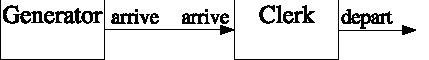
\includegraphics{intro_figs/generator_and_clerk.pdf}
\caption{A block-diagram view of \classname{Generator} and \classname{Clerk} models.}
\label{fig:clerk_and_generator}
\end{figure}

The \classname{Clerk}, \classname{Generator}, and their interconnections constitute a coupled (or network) model. The coupled model depicted in Figure \ref{fig:clerk_and_generator} is realized with a \classname{Digraph} that has the \classname{Generator} and \classname{Clerk} as components. Shown below is the code snippet that creates this two component model.
\begin{verbatim}
int main(int argc, char** argv)
{
    ...
    // Create a digraph model whose components use PortValue<Customer*>
    // objects as input and output objects.
    adevs::Digraph<Customer*> store;
    // Create and add the component models
    Clerk* clrk = new Clerk();
    Generator* genr = new Generator(argv[1]);
    store.add(clrk);
    store.add(genr);
    // Couple the components
    store.couple(genr,genr->arrive,clrk,clrk->arrive);
    ...
\end{verbatim}
This code snippet first creates the components models and then adds them to the \classname{Digraph}. Next, the components are connected by coupling the ``arrive" output port of the \classname{Generator} to the ``arrive" input port of the \classname{Clerk}.

Having created a coupled model to represent the store, all that remains is to perform the simulation. Here is the code snippet that simulates the model.
\begin{verbatim}
...
adevs::Simulator<IO_Type> sim(&store);
while (sim.nextEventTime() < DBL_MAX)
{
    sim.execNextEvent();
}
...
\end{verbatim}
Putting this all of this together gives the main routine for the simulation program that generated the execution traces shown in the example above.
\begin{verbatim}
#include "Clerk.h"
#include "Generator.h"
#include "Observer.h"
#include <iostream>
using namespace std;

int main(int argc, char** argv)
{
    if (argc != 3)
    {
        cout << "Need input and output files!" << endl;
        return 1;
    }
    // Create a digraph model whose components use PortValue<Customer*>
    // objects as input and output objects.
    adevs::Digraph<Customer*> store;
    // Create and add the component models
    Clerk* clrk = new Clerk();
    Generator* genr = new Generator(argv[1]);
    Observer* obsrv = new Observer(argv[2]);
    store.add(clrk);
    store.add(genr);
    store.add(obsrv);
    // Couple the components
    store.couple(genr,genr->arrive,clrk,clrk->arrive);
    store.couple(clrk,clrk->depart,obsrv,obsrv->departed);
    // Create a simulator and run until its done
    adevs::Simulator<IO_Type> sim(&store);
    while (sim.nextEventTime() < DBL_MAX)
    {
        sim.execNextEvent();
    }
    // Done, component models are deleted when the Digraph is
    // deleted.
    return 0;
}
\end{verbatim}

We have completed our first \adevs\ simulation program! However, a few details have been glossed over. The first question - an essential one for a programming language without garbage collection - is what happens to objects that we create in the \classname{Generator} and \classname{Clerk} output functions? The answer is that each model has a garbage collection method that is called at the end of every simulation cycle (in the example above, immediately prior to the return of the method execNextEvent()). The argument to the garbage collection method is a bag of objects created as output in the current simulation cycle.

In our example, the \classname{Clerk} and \classname{Generator} models use their garbage collection method to delete the \classname{Customer} pointed to by each \classname{PortValue} object in the garbage list. The implementation of the garbage collection method is shown below. This listing is for the \classname{Generator} model; the \classname{Clerk}'s \methodname{gc\_output()} method is identical.
\begin{verbatim}
void Generator::gc_output(Bag<IO_Type>& g)
{
    // Delete the customer that was produced as output
    Bag<IO_Type>::iterator i;
    for (i = g.begin(); i != g.end(); i++)
    {
        delete (*i).value;
    }
}
\end{verbatim}

A second question is how to collect the statistics that were our original objective. One approach is to modify the \classname{Clerk} so that it writes waiting times to a file as customers are processed. This approach works but has the unfortunate effect of cluttering up the \classname{Clerk} with code specific to our experiment.

A better approach is to have an \classname{Observer} that is coupled to the \classname{Clerk}'s ``depart" port. The \classname{Observer} records the desired statistics as it receives \classname{Customer} objects on its ``depart" input port. The advantage of this approach is that we can create new types of clerks to perform the same experiment, using, for example, different queuing strategies, without changing the experimental setup (i.e., customer generation and data collection). Similarly, we can change the experiment (i.e., how customers are generated and what data is collected) without changing the clerk.

Below is the code for the \classname{Observer} class. This model is driven solely by external events. The observer reacts to an external event by recording the time that the \classname{Customer} departed the \classname{Clerk}'s queue (i.e., the current simulation time) and how long the \classname{Customer} waited in line. Here is the \classname{Observer} header file.
\begin{verbatim}
#include "adevs/adevs.h"
#include "Customer.h"
#include <fstream>
/**
 * The Observer records performance statistics for a Clerk model
 * based on its observable output.
 */
class Observer: public adevs::Atomic<IO_Type>
{
    public:
        /// Input port for receiving customers that leave the store.
        static const int departed;
        /// Constructor. Results are written to the specified file.
        Observer(const char* results_file);
        /// Internal transition function.
        void delta_int();
        /// External transition function.
        void delta_ext(double e, const adevs::Bag<IO_Type>& xb);
        /// Confluent transition function.
        void delta_conf(const adevs::Bag<IO_Type>& xb);
        /// Time advance function.
        double ta();
        /// Output function.
        void output_func(adevs::Bag<IO_Type>& yb);
        /// Output value garbage collection.
        void gc_output(adevs::Bag<IO_Type>& g);
        /// Destructor.
        ~Observer();
    private:
        /// File for storing information about departing customers.
        std::ofstream output_strm;
};
\end{verbatim}
Below is the \classname{Observer} source file.
\begin{verbatim}
#include "Observer.h"
using namespace std;
using namespace adevs;

// Assign a locally unique number to the input port
const int Observer::departed = 0;

Observer::Observer(const char* output_file):
Atomic<IO_Type>(),
output_strm(output_file)
{
    // Write a header describing the data fields
    output_strm << "# Col 1: Time customer enters the line" << endl;
    output_strm << "# Col 2: Time required for customer checkout" << endl;
    output_strm << "# Col 3: Time customer leaves the store" << endl;
    output_strm << "# Col 4: Time spent waiting in line" << endl;
}

double Observer::ta()
{
    // The Observer has no autonomous behavior, so its next event
    // time is always infinity.
    return DBL_MAX;
}

void Observer::delta_int()
{
    // The Observer has no autonomous behavior, so do nothing
}

void Observer::delta_ext(double e, const Bag<IO_Type>& xb)
{
    // Record the times at which the customer left the line and the
    // time spent in it.
    Bag<IO_Type>::const_iterator i;
    for (i = xb.begin(); i != xb.end(); i++)
    {
        const Customer* c = (*i).value;
        // Compute the time spent waiting in line
        double waiting_time = (c->tleave-c->tenter)-c->twait;
        // Dump stats to a file
        output_strm << c->tenter << " " << c->twait << " " <<
            c->tleave << " " << waiting_time << endl;
    }
}

void Observer::delta_conf(const Bag<IO_Type>& xb)
{
    // The Observer has no autonomous behavior, so do nothing
}

void Observer::output_func(Bag<IO_Type>& yb)
{
    // The Observer produces no output, so do nothing
}

void Observer::gc_output(Bag<IO_Type>& g)
{
    // The Observer produces no output, so do nothing
}

Observer::~Observer()
{
    // Close the statistics file
    output_strm.close();
}
\end{verbatim}

This model is coupled to the \classname{Clerk}'s ``depart" output port in the same manner as before. The resulting coupled model is illustrated in Figure \ref{fig:complete_store_model}.
\begin{figure}[ht]
\centering
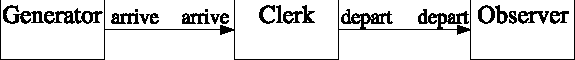
\includegraphics{intro_figs/generator_and_clerk_and_observer.pdf}
\caption{The \classname{Generator}, \classname{Clerk}, and \classname{Observer} model.}
\label{fig:complete_store_model}
\end{figure}

Given the customer arrival data in Table \ref{tab:customer_data}, the consequent customer departure and waiting times are shown in Table \ref{tab:simulation_output}. With this output, we can use a spreadsheet to find the maximum and average times that the customers spent waiting in line.
\begin{table}
\centering
\begin{tabular}{|c|c|}
\hline
Time that the customer left the store & Time spent waiting in line \\ \hline
2 & 0 \\ \hline
6 & 0 \\ \hline
10 & 3 \\ \hline
12 & 5 \\ \hline
22 & 5 \\ \hline
42 & 14 \\ \hline
44 & 32 \\ \hline
45 & 33 \\ \hline
\end{tabular}
\caption{Customer departure times and waiting times.}
\label{tab:simulation_output}
\end{table}

Again notice that the customer departure times correspond exactly with the production of customer departure events by the \classname{Clerk} model. Each entry in Table \ref{tab:simulation_output} is the result of executing the \classname{Observer}'s external transition function. Also notice that the \classname{Observer}'s internal and confluent transition functions are never executed because the \classname{Observer}'s time advance method always returns infinity.

This section has demonstrated the most common parts of a simulation program built with \adevs. The remainder of the manual covers \classname{Atomic} and \classname{Network} models in greater detail, demonstrates the construction of variable structure models, and shows how continuous models can be added to your discrete event simulation.
